
%(BEGIN_QUESTION)
% Copyright 2010, Tony R. Kuphaldt, released under the Creative Commons Attribution License (v 1.0)
% This means you may do almost anything with this work of mine, so long as you give me proper credit

Suppose a voltmeter registers 0 volts between test points {\bf A} and {\bf D} in this series-parallel circuit:

$$\includegraphics[width=15.5cm]{i01859x01.eps}$$

Determine the diagnostic value of each of the following tests.  Assume only one fault in the system, including any single component or any single wire/cable/tube connecting components together.  If a proposed test could provide new information to help you identify the location and/or nature of the one fault, mark ``yes.''  Otherwise, if a proposed test would not reveal anything relevant to identifying the fault (already discernible from the measurements and symptoms given so far), mark ``no.''

% No blank lines allowed between lines of an \halign structure!
% I use comments (%) instead, so that TeX doesn't choke.

$$\vbox{\offinterlineskip
\halign{\strut
\vrule \quad\hfil # \ \hfil & 
\vrule \quad\hfil # \ \hfil & 
\vrule \quad\hfil # \ \hfil \vrule \cr
\noalign{\hrule}
%
% First row
{\bf Diagnostic test} & {\bf Yes} & {\bf No} \cr
%
\noalign{\hrule}
%
% Another row
Measure $V_{CD}$ with power applied &  &  \cr
%
\noalign{\hrule}
%
% Another row
Measure $V_{DF}$ with power applied &  &  \cr
%
\noalign{\hrule}
%
% Another row
Measure $V_{DE}$ with power applied &  &  \cr
%
\noalign{\hrule}
%
% Another row
Measure $I_{R1}$ with power applied &  &  \cr
%
\noalign{\hrule}
%
% Another row
Measure $I_{R2}$ with power applied &  &  \cr
%
\noalign{\hrule}
%
% Another row
Measure $R_{AB}$ with source disconnected from {\bf C} &  &  \cr
%
\noalign{\hrule}
%
% Another row
Measure $R_{DF}$ with source disconnected from {\bf E} &  &  \cr
%
\noalign{\hrule}
%
% Another row
Measure $R_{CF}$ with source disconnected from {\bf C} &  &  \cr
%
\noalign{\hrule}
%
% Another row
Measure $R_{CD}$ with wire disconnected between {\bf A} and {\bf C} &  &  \cr
%
\noalign{\hrule}
%
% Another row
Measure $R_{CD}$ with $R_3$ disconnected from {\bf D} &  &  \cr
%
\noalign{\hrule}
} % End of \halign 
}$$ % End of \vbox

\vfil 

\underbar{file i01859}
\eject
%(END_QUESTION)





%(BEGIN_ANSWER)

% No blank lines allowed between lines of an \halign structure!
% I use comments (%) instead, so that TeX doesn't choke.

$$\vbox{\offinterlineskip
\halign{\strut
\vrule \quad\hfil # \ \hfil & 
\vrule \quad\hfil # \ \hfil & 
\vrule \quad\hfil # \ \hfil \vrule \cr
\noalign{\hrule}
%
% First row
{\bf Diagnostic test} & {\bf Yes} & {\bf No} \cr
%
\noalign{\hrule}
%
% Another row
Measure $V_{CD}$ with power applied & $\surd$ &  \cr
%
\noalign{\hrule}
%
% Another row
Measure $V_{DF}$ with power applied & $\surd$ &  \cr
%
\noalign{\hrule}
%
% Another row
Measure $V_{DE}$ with power applied & $\surd$ &  \cr
%
\noalign{\hrule}
%
% Another row
Measure $I_{R1}$ with power applied & $\surd$ &  \cr
%
\noalign{\hrule}
%
% Another row
Measure $I_{R2}$ with power applied & $\surd$ &  \cr
%
\noalign{\hrule}
%
% Another row
Measure $R_{AB}$ with source disconnected from {\bf C} & $\surd$ &  \cr
%
\noalign{\hrule}
%
% Another row
Measure $R_{DF}$ with source disconnected from {\bf E} & $\surd$ &  \cr
%
\noalign{\hrule}
%
% Another row
Measure $R_{CF}$ with source disconnected from {\bf C} & $\surd$ &  \cr
%
\noalign{\hrule}
%
% Another row
Measure $R_{CD}$ with wire disconnected between {\bf A} and {\bf C} &  & $\surd$ \cr
%
\noalign{\hrule}
%
% Another row
Measure $R_{CD}$ with $R_3$ disconnected from {\bf D} & $\surd$ &  \cr
%
\noalign{\hrule}
} % End of \halign 
}$$ % End of \vbox

Remember, it is {\it always} useless to measure resistance where there exists significant voltage in a circuit!

%(END_ANSWER)





%(BEGIN_NOTES)


%INDEX% Troubleshooting review: electric circuit diagnostic test usefulness

%(END_NOTES)


